\chapter{基于RNN的深度强化学习混合模型在直复营销中的建模}
% 首先介绍直复营销问题使用强化学习研究的现状(函数逼近存在的问题,以及现行的解决方案和思路,从而引出本文的方法思路)
% 介绍深度强化学习
% 介绍本文提出的混合网络模型算法


\section{直复营销问题概述}
直复营销是客户关系管理中的一项重要内容,它需要企业长时间的与客户进行营销交互,以此来判断客户的对营销产品的喜好,进而可以辅助企业进行营销活动,增加企业的收入。具体来说,在每个需要进行营销的时刻点,企业会对客户采取营销行为,比如发送宣传单、促销邮件或者优惠券等等,作为反馈,客户可能会访问该企业资讯相关产品或者会下一定金额的订单又或者是简单的忽略掉此次的营销活动。所以,企业需要在营销的时候决定对那些客户进行营销行为,可以使的企业的收益最大。

在直复营销中,企业在某一时刻对某一客户采取的营销行为可能会对用户未来的反馈行为产生影响。也就是说,营销行为对用户的营销是长期的并且用户的反馈也可能是延迟的。所以,企业通常把最大化用户生命周期的价值(life-time value, LTV)作为评价营销效果的指标\citep{dwyer1997customer}。那么,直复营销问题就可以自然的表述为一个基本的强化学习问题,其中,即时利润看作是回报,LTV作为长期的价值函数。文献\citep{tkachenko2015autonomous,pednault2002sequential,silver2013concurrent}都是以此想法为出发点,将强化学习应用在广告营销中,并且取得了较好的表现。

然而,像诸如机器人和人机交互等其它现实应用所面临的问题一样,在直复营销场景中,因为客户状态(马尔科夫状态)的部分可观测性使的这一问题很具有挑战性。在理想的马尔科夫决策过程中,一个客户的状态就可以概括他和该企业在此之前的整个交互历史,也就是说客户的未来响应情况与之前的交互历史无关,只与在当前状态和未来的行为有关。然而,在直复营销这种复杂的现实场景中,构建和衡量这种状态是很难的。即使像在直复营销中比较流行的Recency-Frequency-Monetary价值模型,也仅仅捕获到了客户真实状态中的部分信息。因此,对这些场景使用强化学习之前,进行状态的推理是很重要的。

在强化学习的研究和应用中,处理部分可观测状态最常用的方法就是使用部分可观测的马尔科夫决策过程(Partially Observable Markov decision Process,POMDP)\citep{kaelbling1998planning},并且已经在一些诸如机器人、人机对话等领域取得了不错的表现。但是,在POMDP中对隐状态的定义需要大量的领域知识,而获取这些领域知识在一些复杂的现实应用中是很难获得的。
% 在POMDP中,因为agent对环境观测的局限性,所以多了一步agent对当前所处状态可信度的判断。即根据环境观测信息来判断agent的状态是有偏差的,这种偏差用概率来表示就是agent对自己目前所处状态的可信度有多大。

受深度强化学习成功应用在游戏、围棋等领域的启发,我们考虑使用深度神经网络来来自动捕捉和推断系统的隐含状态。与POMDP不同的是,深度神经网络可以对给定问题自动的给出适当的表示,从而可以解决在设计隐状态时遇到的困难和挑战,这对与专家来说是很难办到的。以上本文选择使用深度强化学习解决直复营销问题的出发点,特别的,我们对现有的网络结构做了近一步的改进优化。

\section{深度强化学习DQN}
\subsection{Q-learning回顾}
在算法$\ref{algo:algorithm_2}$中,我们对Q-learning方法做了详细介绍,Q-learning方法主要思想是异策略的时间差分方法。

异策略,就是指的行为策略(产生数据的策略)和要评估的策略不是一个策略。在Q-learning中,行为策略是第6行的$\epsilon-greedy$的策略,而用于评估和改善的策略是第7行的贪婪策略(每个状态取值函数最大的那个行为)。

时间差分方法,是指利用时间差分目标来更新当前行为的值函数。在Q-learning中,时间差分的目标就是$r+\gamma \max_{a} Q(s^{'},a^{'})$。
\subsection{DQN}
 深度强化学习以DQN最为代表性,它就是在Q-learning的基础上修改得到的,主要进行了以下三个方面的改进。

 \paragraph{利用卷积神经网络逼近值函数}
 DQN利用深度卷积神经网络逼近值函数。如图\ref{fig:CNN_DQN}所示为状态行为值函数的逼近网络结构。利用神经网络逼近值函数属于参数化的非线性逼近方法,不仅具有很强的表征能力,而且还可以自动的捕捉到环境的隐状态信息。此处的值函数对应着一组参数,也就是神经网络中每层网络的参数,我们可以用向量$\mathbf{\theta}$表示,对应的值函数可以表示为$Q(s,a;\mathbf{\theta})$,所以对值函数的更新也就是对参数向量$\mathbf{\theta}$,当网络结构确定后,$\mathbf{\theta}$就代表着值函数。DQN所使用的网络结构是三个卷基层加两个全连阶层。
\begin{figure}[htbp]
\centering
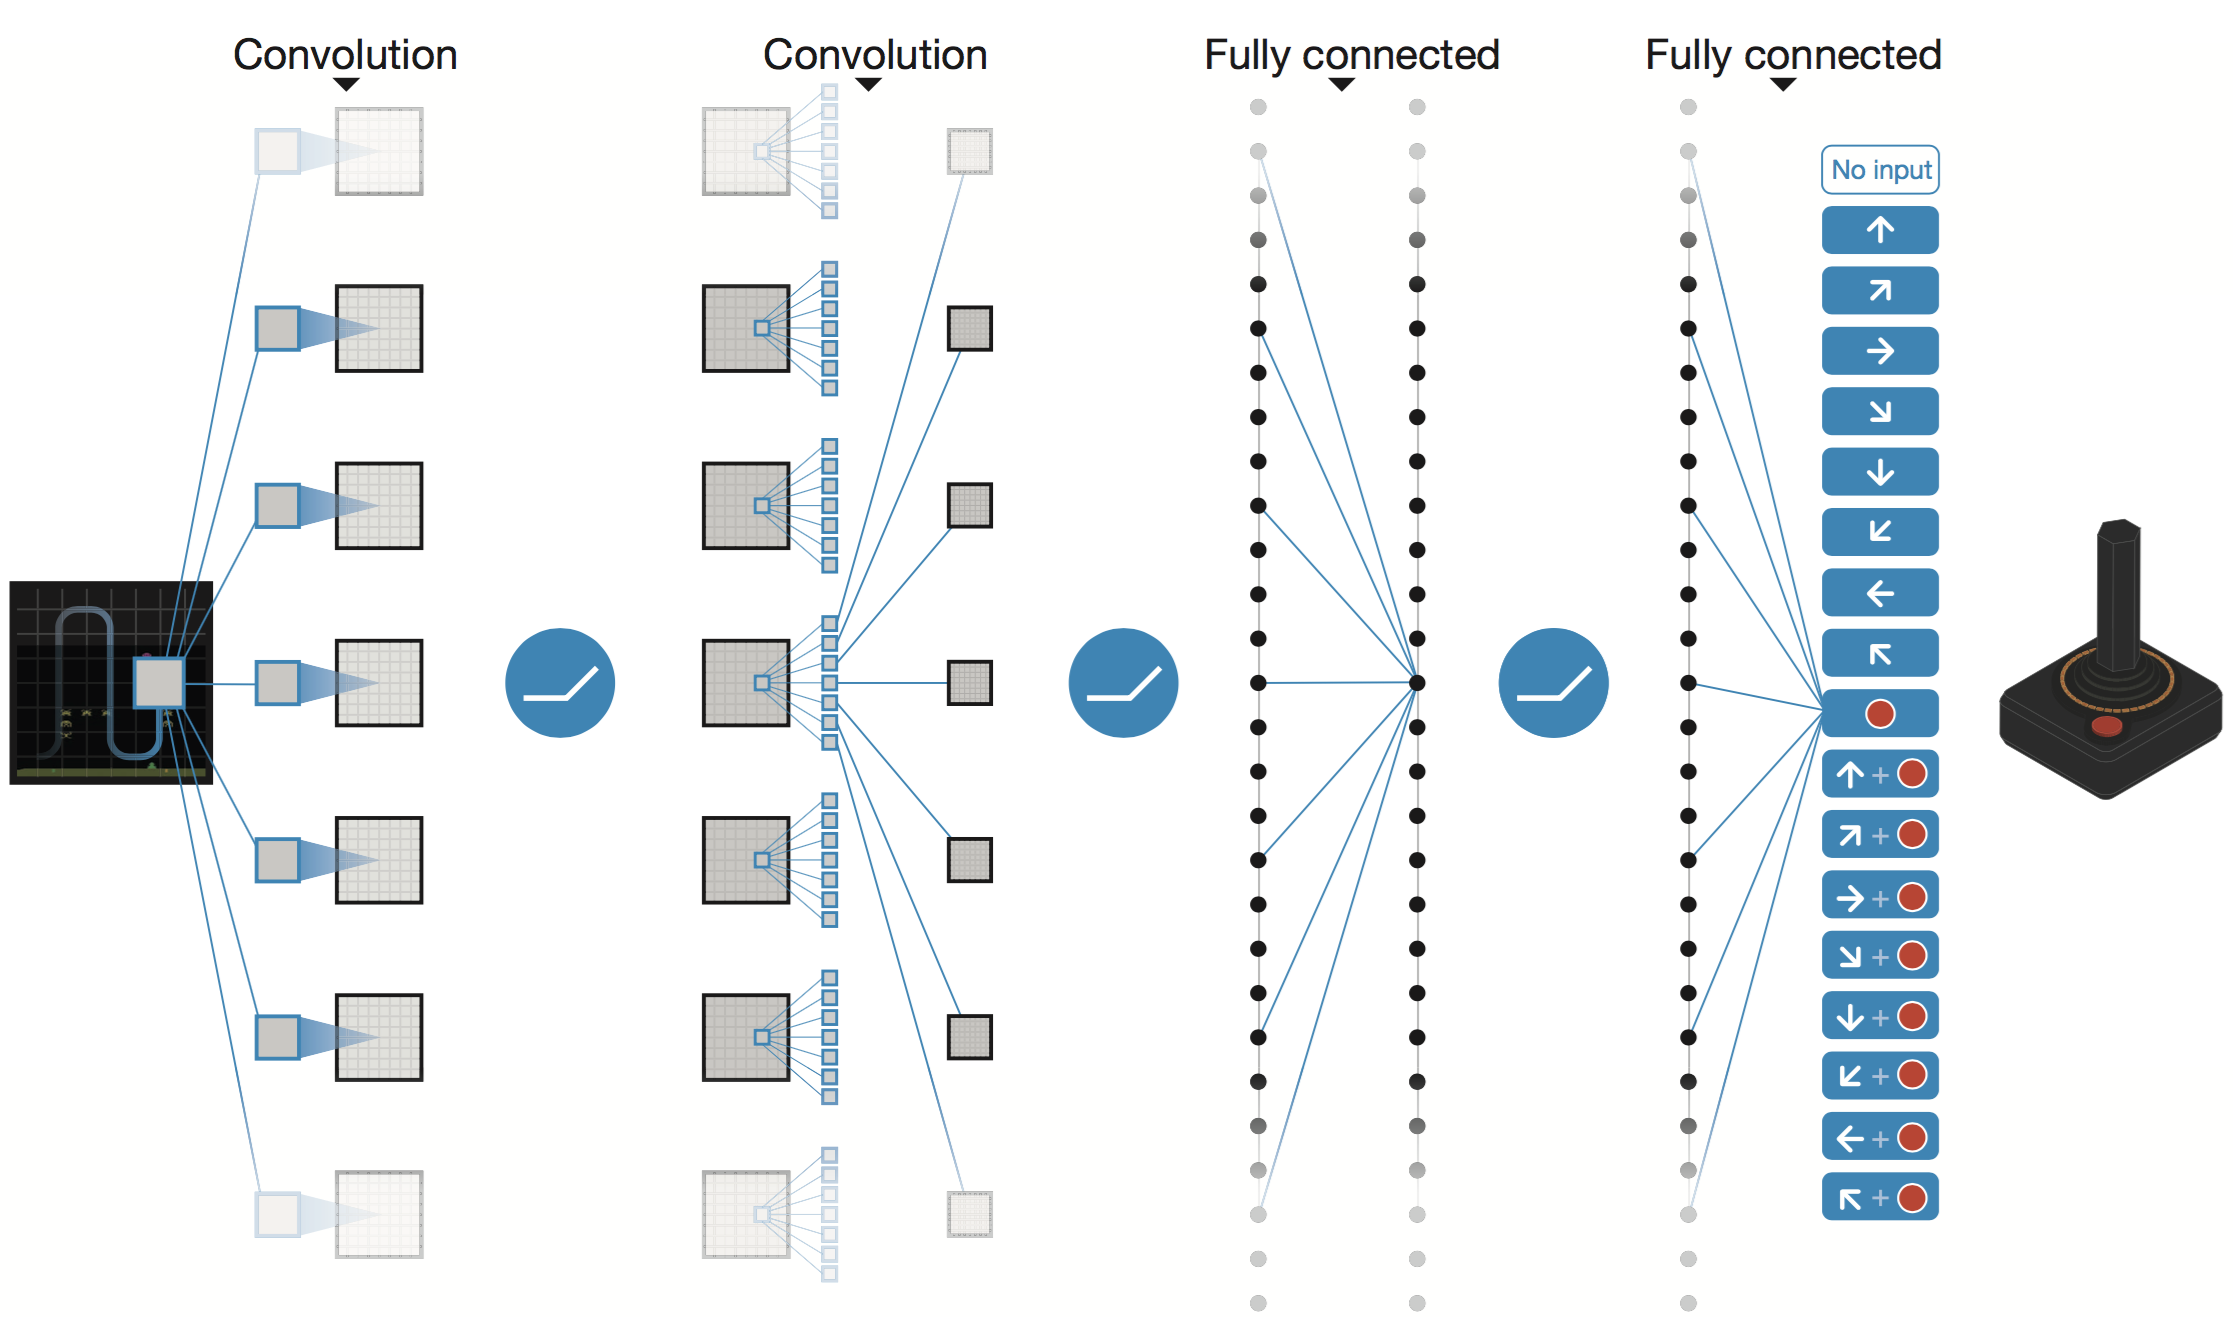
\includegraphics[width=1.0\textwidth]{CNN_DQN}
\caption{DQN状态行为值函数逼近网络}
\label{fig:CNN_DQN}
\end{figure}

其实,1995年Bertsekas等人最早将神经网络应用在在强化学习的值函数逼近中,取得了相比线性逼近较好的结果,但是往往会出现不稳定不收敛的情况\citep{bertsekas1995neuro}。此后,众多学者在这个方向上一直没有突破,直到DeepMind团队的出现。

 \paragraph{设置经验回放机制}
DeepMind团队的创始人Hassabis是神经科学的博士,他主要研究人类大脑中的海马体,海马体是大脑中主要负责记忆和学习的部分。他在研究时发现,人类在睡觉的时候,海马体会把一天的记忆重放给大脑皮层,利用这个启发机制,DeepMind团队的研究人员设计了一种神经网络的训练方法:经验回放。

经验回放是指,在强化学习的过程中,agent将数据存储在一个数据库中,再利用均匀采样的方法从数据库中抽取数据,然后利用抽取的数据训练神经网络。通过这种方法可以使的神经网络训练收敛且稳定。因为在训练神经网络时,我们假设的前提是训练数据是独立同分不的,但是通过强化学习采集的数据之间存在关联性,利用这些数据进行顺序训练,神经网络难免会不稳定。但是利用经验回放可以打破这种数据间的关联性。

 \paragraph{设置独立的目标网络}
与表格型Q-learning强化学习算法不同的是,利用神经网络对值函数进行逼近时,对值函数的更新其实就是对参数向量$\mathbf{\theta}$的更新,其更新方法时梯度下降法,因此算法$\ref{algo:algorithm_2}$第7行值函数的更新实际上变成了进度学习的一次更新过程,其梯度下降法为:
\begin{displaymath}
\begin{aligned}
\mathbf{\theta}_{t+1}=\mathbf{\theta}_{t}+\alpha[r+\gamma \max_{s^{'}}Q(s^{'},a^{'};\mathbf{\theta})-Q(s,a;\mathbf{\theta})]\triangledown Q(s,a;\mathbf{\theta})
\end{aligned}
\end{displaymath}
其中,$r+\gamma \max_{s^{'}}Q(s^{'},a^{'};\mathbf{\theta}$为TD目标,在计算$\max_{s^{'}}Q(s^{'},a^{'};\mathbf{\theta}$时用到的参数向量为$\mathbf{\theta}$。

我们称计算TD目标时所用的网络为TD网络。在DQN算法出现之前,利用神经网络逼近值函数时,计算TD目标的状态行为值函数所用的网络参数$\mathbf{\theta}$,与梯度计算中要逼近的值函数所用的网路参数向量相同,这样就容易导致数据间存在关联性,从而使训练不稳定。为了解决此问题,DeepMind提出计算TD目标的网络参数为$\mathbf{\theta}^{-}$,计算值函数逼近网络表示为$\mathbf{\theta}$;用于状态行为值函数逼近的网络每一步都要更新,而用于计算目标的网络则是每个固定的步骤更新一次。

因此,值函数的更新变为:
\begin{displaymath}
\begin{aligned}
\mathbf{\theta}_{t+1}=\mathbf{\theta}_{t}+\alpha[r+\gamma \max_{s^{'}}Q(s^{'},a^{'};\mathbf{\theta^{-}})-Q(s,a;\mathbf{\theta})]\triangledown Q(s,a;\mathbf{\theta})
\end{aligned}
\end{displaymath}

 \paragraph{DQN框架}
 由此,我们可以得到DQN的算法流程图$\ref{fig:liuchengtu_DQN}$:
\begin{figure}[htbp]
\centering
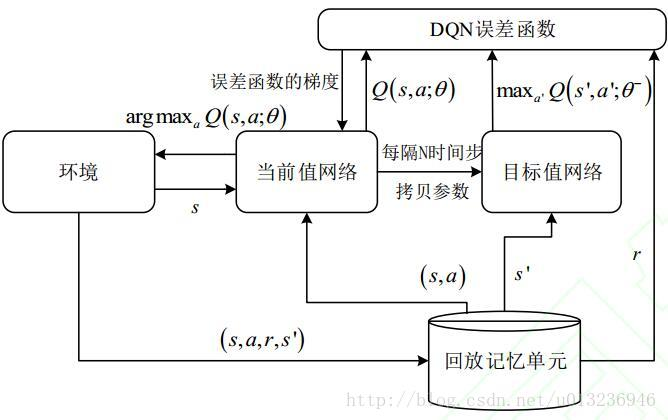
\includegraphics[width=0.9\textwidth]{liuchengtu_DQN}
\caption{DQN流程图}
\label{fig:liuchengtu_DQN}
\end{figure}

DQN的损失函数构造$\ref{fig:liuchengtu_DQN}$:
\begin{figure}[htbp]
\centering
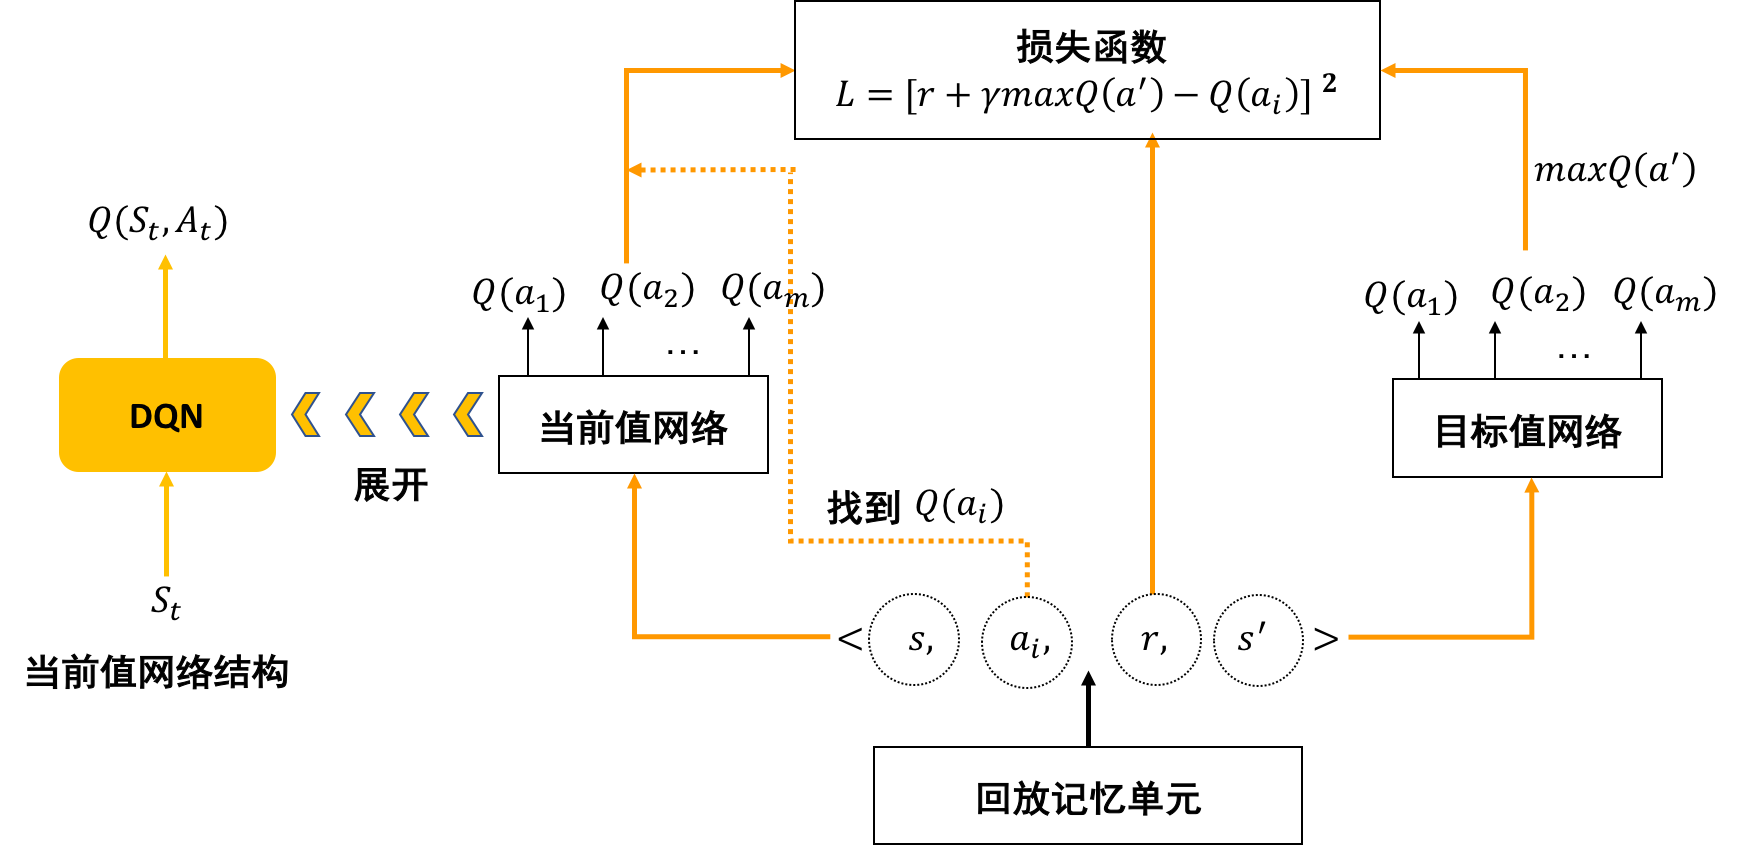
\includegraphics[width=0.8\textwidth]{loss_DQN}
\caption{DQN损失函数构造}
\label{fig:loss_DQN}
\end{figure}

结合算法$\ref{algo:algorithm_2}$,我们可以得到DQN伪代码为算法$\ref{algo:algorithm_DQN}$:
\begin{algorithm}[htbp]
\small
\SetAlgoLined
\SetKwRepeat{Repeat}{repeat}{until} 
初始化回放记忆库$D$,记忆库大小为$N$\;
利用随机权值$\mathbf{\theta}$初始化状态行为值函数$Q$\;
初始化$\mathbf{\theta}^{-}$令$\mathbf{\theta}^{-}=\mathbf{\theta}$,用以计算TD目标的状态行为值$\hat{Q}$\;
\For{$episode=1,\cdots, M$}{
	初始化情节的第一个状态:$s_{1}={x_{1}}$(${x_{1}}$为环境的观测特征),通过预处理得到状态对应的特征输入:$\phi_{1}=\phi(s_{1})$\;
	\For{$t=1,\cdots, T$}{
		以概率$\epsilon$选一个随机行为$a_{t}$\;
		如果以上小概率事件没有发生,则按照贪婪策略选择当前值函数最大的那个行为:$a_{t}=\argmax_{a}Q(\phi(s_{t}),a;\mathbf{\theta})$\;
		在仿真器中执行行为$a_{t}$,可以观测到奖赏$r_{t}$以及下一步的环境的观测特征\;
		设置$s_{t+1}=s_{t},a_{t},x_{t+1}$,预处理得到对应的特征输入:$\phi_{t+1}=\phi(s_{t+1})$\;
		将转换样本($\phi_{t}, a_{t}, r_{t}, \phi(s_{t+1})$)到回放记忆库中\;
		从回放记忆库D中均匀随机采样一个转换样本数据($\phi_{j}, a_{j}, r_{j}, \phi(s_{j+1})$)\;
		判断是否是一个情节的终止状态,若是,则TD目标位$r_{j}$,否则利用TD目标网络$\mathbf{\theta}^{-}$计算TD目标$r+\gamma \max_{s^{'}}Q(s^{'},a^{'};\mathbf{\theta^{-}})$\;
		执行一次梯度下降算法:$\triangle \theta = \alpha (v_{\pi}(s)-\hat{v}(s,\mathbf{\theta})) \triangledown_{\theta} \hat{v}(s,\mathbf{\theta})$\;
		更新状态行为值函数逼近的网络参数:$\mathbf{\theta}=\mathbf{\theta}+\triangle \theta$\;
		每隔$C$步更新一次TD目标网络权值;即:$\mathbf{\theta}^{-}=\mathbf{\theta}$\;
	}
}
% 输出最终策略:$\pi(s)=\argmax_{a}Q(s,a)$\;
\caption{DQN伪代码}
\label{algo:algorithm_DQN}
\end{algorithm}


\section{基于LSTM的深度强化学习混合模型设计}
\subsection{RNN和LSTM}
\subsection{混合模型}
\subsection{两步混合模型}
\subsection{其它对照实验模型}


\section{本章小结}